%% all trees of order 1
\subfigure[$n = 1$]{
\begin{tikzpicture}
[nodedecorate/.style={shape=circle,inner sep=2pt,draw,thick},%
  linedecorate/.style={-,thick}]
\node () at (0,0) [nodedecorate] {};
%% buffer nodes; these should not be visible
\node () at (-0.5,0) [] {};
\node () at (0.5,0) [] {};
\end{tikzpicture}
}
\quad
%%
%% all trees of order 2
\subfigure[$n = 2$]{
\begin{tikzpicture}
[nodedecorate/.style={shape=circle,inner sep=2pt,draw,thick},%
  linedecorate/.style={-,thick}]
%% nodes or vertices
\foreach \nodename/\x/\y in {1/0/0, 2/0/1} {
  \node (\nodename) at (\x,\y) [nodedecorate] {};
}
%% buffer nodes; these should not be visible
\node () at (-0.5,0) [] {};
\node () at (0.5,0) [] {};
%% edges or lines
\path
(1) edge[linedecorate] node {} (2);
\end{tikzpicture}
}
\quad
%%
%% all trees of order 3
\subfigure[$n = 3$]{
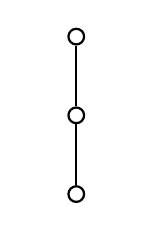
\begin{tikzpicture}
[nodedecorate/.style={shape=circle,inner sep=2pt,draw,thick},%
  linedecorate/.style={-,thick}]
%% nodes or vertices
\foreach \nodename/\x/\y in {1/0/0, 2/0/1, 3/0/2} {
  \node (\nodename) at (\x,\y) [nodedecorate] {};
}
%% buffer nodes; these should not be visible
\node () at (-0.5,0) [] {};
\node () at (0.5,0) [] {};
%% edges or lines
\path
\foreach \startnode/\endnode in {1/2, 2/3} {
  (\startnode) edge[linedecorate] node {} (\endnode)
};
\end{tikzpicture}
}
